\documentclass{beamer}
\mode<presentation> {
\usetheme{Madrid}
}

\usepackage{amsmath,amsthm,amssymb,amsfonts,cancel}
\usepackage{graphicx} % Allows including images
\usepackage{color}

\usepackage{booktabs} % Allows the use of \toprule, \midrule and \bottomrule in tables
\usepackage{caption}
\usepackage{algorithm} 
\usepackage{algpseudocode}
%\usepackage[style=verbose, backend=bibtex,maxcitenames=4]{biblatex}
%\addbibresource{references.bib}
%{\footnotesize
%\bibliography{references}}

%%change footnotecite
%\renewcommand*{\thefootnote}{[\arabic{footnote}]}
%\makeatletter
%% Remove superscript for footnotemark
%\def\@makefnmark{\hbox{{\normalfont\@thefnmark}}}
%% Allow space to precede the footnote
%\usepackage{etoolbox}
%\patchcmd{\blx@mkbibfootnote}{\unspace}{}{}
%\makeatother
\usepackage{bbm}
\usepackage{natbib} 
\setbeamertemplate{bibliography item}{}
\setbeamertemplate{theorems}[numbered]
\newtheorem{thm}{Theorem}
\newtheorem{lem}[thm]{Lemma}
\newtheorem{cor}{Corollary}
\newtheorem*{defi*}{Definition}
\newcommand{\G}{\mathcal{G}}
\providecommand{\mb}[1]{\boldsymbol{#1}}
\newcommand{\Real}{\mathbb{R}}

\title[JSM2016]{Dependence Discovery from Multimodal Data via Multiscale Graph Correlation} 

\author{Cencheng Shen} % Your name
\institute[Temple University] % Your institution as it will appear on the bottom of every slide, may be shorthand to save space
{
\textit{Joint Work with Joshua T. Vogelstein \& Mauro Maggioni \& Carey E. Priebe} \\
%\medskip
%Department of Statistics \\
%Temple University \\  % Your institution for the title page
}
\date{August, 2016} % Date, can be changed to a custom date

\AtBeginSection{\frame{\sectionpage}}

\begin{document}
\bibliographystyle{plainnat}
\begin{frame}
\titlepage % Print the title page as the first slide
\end{frame}
%1. Intro; 2. it is linear regression and classification; 3. its origin, and why we start investigation; 4. explain title

\begin{frame}
\frametitle{Overview} % Table of contents slide, comment this block out to remove it
\tableofcontents % Throughout your presentation, if you choose to use \section{} and \subsection{} commands, these will automatically be printed on this slide as an overview of your presentation
\end{frame}

\section{Motivations}
\begin{frame}{Motivations}
\begin{itemize}[<+->]
\item Given multiple data sets, we would like to test whether they are independent or not.
\item Modern data sets may be high-dimensional, nonlinear, noisy, of small sample size; and different data sets may come from disparate spaces.
\item In particular, we are investigating the association between brain activities and various phenotypes, such as brain Connectome vs certain disease, or brain vs personality, where the brain data is usually obtained via fMRI scans for a number of brain regions at consecutive time steps.
\item Before we try all kinds of regression / classification methods, the first task is to determine whether there exists strong dependency for given pair of data.
\end{itemize}
\end{frame}

\begin{frame}
\begin{itemize}[<+->]
\item \textbf{How to reliably test independence on given data?}
\item We would like a test statistic that:
\item 1) is consistent as the sample size increases to infinity for all dependencies.
\item 2) has a good finite-sample testing power, for given data of low or high dimensionality, linear or non-linearity, small sample size, with noise, etc.
\item 3) provides insight into the dependency structure
\item 4) does not inflate the false positive rate in the absence of dependency.
\item 5) easy to use and scalable on big data
\item To that end, we propose multiscale graph correlation in \cite{ShenEtAl2016} for testing independence, which combines distance correlation and nearest-neighbor into the same testing framework.
\end{itemize}
\end{frame}

\section{Results}
\subsection{Global Correlation Coefficient}
\begin{frame}{General Correlation Coefficient}
A general correlation coefficient $\G$ can be expressed as follows:
\begin{equation}
\label{generalCoef}
\G=\frac{\sum_{i,j=1}^n (a_{ij}-\bar{a}) (b_{ij}-\bar{b})}{\sqrt{\sum_{i,j=1}^n  (a_{ij}-\bar{a})^{2} \sum_{i,j=1}^n (b_{ij}-\bar{b})^{2}}}, 
\end{equation}
where $\bar{a}$ and $\bar{b}$ denote the sample means of $a_{ij}$ and $b_{ij}$.
\end{frame}

\begin{frame}{Examples}
\begin{itemize}[<+->]
\item Suppose $X=[x_{1},\cdots, x_{n}] \in \Real^{d_{x} \times n}$ and $Y=[y_{1},\cdots, y_{n}] \in \Real^{d_{y} \times n}$ are the corresponding data sets.
\item The Pearson's correlation coefficient can be calculated by taking $a_{ij}=x_i$ and $b_{ij}=y_i$.
\item Spearman and Kendall's rank correlations set $a_{ij}$ to be $rank(x_i)-rank(x_j)$ and $sign(x_i-x_j)$.
\item The Mantel coefficient \cite{Mantel1967} considers distance matrices and takes $a_{ij}=|x_i-x_j|_{2}$.
\item The distance correlation (dcorr) proposed in \cite{SzekelyRizzoBakirov2007} uses the doubly-centered distance entries for $a_{ij}$ and $b_{ij}$.
\item The modified distance correlation (mcorr) proposed in \cite{SzekelyRizzo2013a} slightly modifies $a_{ij}/b_{ij}$ of dcorr to make the resulting $\G$ unbiased.
\end{itemize}
\end{frame}

\subsection{Local Correlation Coefficients}
\begin{frame}{Local Correlation}
\begin{itemize}[<+->]
\item We combine nearest-neighbor into global correlation, by defining a family of local correlation coefficients.
\item Let $rank(a_{ij})$  be the ``rank'' of $x_i$ relative to $x_j$, that is, $rank(a_{ij})=k$ if $x_i$ is the $k^{th}$ closest point (or ``neighbor'') to $x_j$; and the ranks start from $k=1$ onwards (i.e., $rank(a_{jj})=1$), and the minimal rank is used for ties. 
\item Then for any general correlation coefficient $\G$ in the form of Equation~\ref{generalCoef}, we define its \emph{local} variants by
\begin{equation}
\label{localCoef}
\G_{kl}=\frac{\sum_{i,j=1}^n (a_{ij}^k-\bar{a}^{k}) (b_{ij}^l-\bar{b}^{l})}{\sqrt{\sum_{i,j=1}^n  (a_{ij}^{k}-\bar{a}^{k})^2 \sum_{i,j=1}^n (b_{ij}^{l}-\bar{b}^{l})^2}},
\end{equation}
for $k=1,\ldots,\max(rank(a_{ij}))$, $l=1,\ldots,\max(rank(b_{ij}))$, where
\begin{equation}
\label{localCoef2}
    a_{ij}^k=
    \begin{cases}
      a_{ij}, & \text{if } 0 < rank(a_{ij}) \leq k, \\
      0, & \text{otherwise};
    \end{cases} \qquad \qquad
    b_{ij}^l=
    \begin{cases}
      b_{ij}, & \text{if } 0 < rank(b_{ij}) \leq l, \\
      0, & \text{otherwise};
    \end{cases}
\end{equation}
\end{itemize}
\end{frame}

\subsection{Multiscale Graph Correlation}
\begin{frame}{MGC}
\begin{itemize}[<+->]
\item In the family of local correlations $\{\G_{kl}\}$, there always exists an optimal local correlation with respect to the independence testing power. 
\item The optimal scale exists, is distribution dependent, and may not be unique.
\item We dub the optimal local correlation coefficient as the multiscale graph correlation, and denote it as $\G^{*}$.
\item Although each local correlation requires $O(n^2)$ to compute, we provide a fast algorithm to compute all local correlations simultaneously in $O(n^2)$, assuming the rank information is given (note: sorting the distance matrix column-wise takes $O(n^2 \log(n))$).
\item This allows the optimal scale to be efficiently determined for MGC, unlike many other applications by nearest-neighbor (say knn classification, manifold learning, etc.).
\end{itemize}
\end{frame}

\begin{frame}{The Testing Framework}
\begin{itemize}[<+->]
\item Given two data sets $X=[x_{1},\cdots, x_{n}] \in \mathcal{R}^{d_{X} \times n}$ and $Y=[y_{1},\cdots, y_{n}] \in \mathcal{R}^{d_{Y} \times n}$.
\item Assume that $x_{i}, i=1,\ldots,n$ are identically independently distributed (i.i.d.) as $\mb{x} \sim f_{x}$; similarly each $y_{i}$ are realizations of $\mb{y} \sim f_{y}$. 
\item The null and the alternative hypothesis for testing independence are
\begin{align*}
& H_{0}: f_{xy}=f_{x}f_{y},\\
& H_{A}: f_{xy} \neq f_{x}f_{y},
\end{align*}
where $f_{xy}$ denotes the joint distribution of $(\mb{x},\mb{y})$. 
\item For a given pair of data with unknown model, we can use the permutation test, and reject the null when the p-value is sufficiently small.
\end{itemize}
\end{frame}

\subsection{Theoretical Advantages}
\begin{frame}{Theorems of MGC}
\begin{thm}
\label{thm1}
Multiscale graph correlation is consistent against all dependent alternatives of finite second moments, i.e., $\beta_{\alpha}(\G^{*}) \rightarrow 1$ as $n\rightarrow \infty$ at any type 1 error level $\alpha$, when distance correlation or modified distance correlation is used as the global correlation $\G$.
\end{thm}
\pause
\medskip
\begin{thm}
\label{thm2}
Suppose $\mb{x}$ is linearly dependent of $\mb{y}$. Then for any $n$ and $\alpha$ it always holds that
\begin{equation}
\beta_{\alpha}(\G^{*}) = \beta_{\alpha}(\G).
\end{equation}

Thus multiscale graph correlation is equivalent to the global correlation coefficient under linear dependency.
\end{thm}

\end{frame}

\begin{frame}{Theorems of MGC}
\begin{thm}
\label{thm3}
There exists $f_{xy}$, $n$ and $\alpha$ such that 
\begin{equation}
\beta_{\alpha}(\G^{*}) > \beta_{\alpha}(\G).
\end{equation}

Thus multiscale graph correlation can be better than its global correlation coefficient under certain nonlinear dependency.
\end{thm}
We use a quadratic relationship and finite $n$ to prove theorem~\ref{thm3}.
\end{frame}

\subsection{Numerical Experiments}
\begin{frame}{Simulation Set-Up}
\begin{itemize}[<+->]
\item In total $20$ different distributions of $f_{xy}$ are considered, most of which are based on simulations from existing literature.
\item They consist of various linear and close to linear dependencies (e.g., exponential, joint normal), polynomial-based nonlinear relationships (e.g., quadratic, fourth-root), trigonometry-based nonlinear dependencies (e.g., circle, spiral), two uncorrelated but dependent dependencies, and an independent relationship. 
\item For each distribution, we further consider two different scenarios: a $1$-dimensional scenario with increasing sample size, and a high-dimensional scenario with fixed sample size but increasing dimensions.
\item The benchmarks are distance correlation, modified distance correlation, the Mantel test, and the HHG method proposed in \cite{HellerGorfine2013}.
\item To better illustrate the effectiveness of distance-based local correlation, we consider three MGC implementations by dcorr / mcorr / Mantel respectively in the simulation.
\end{itemize}
\end{frame}

\begin{frame}{Visualization of Sample Data for Each Joint Distribution}
\begin{figure}[ht]
  \centering
  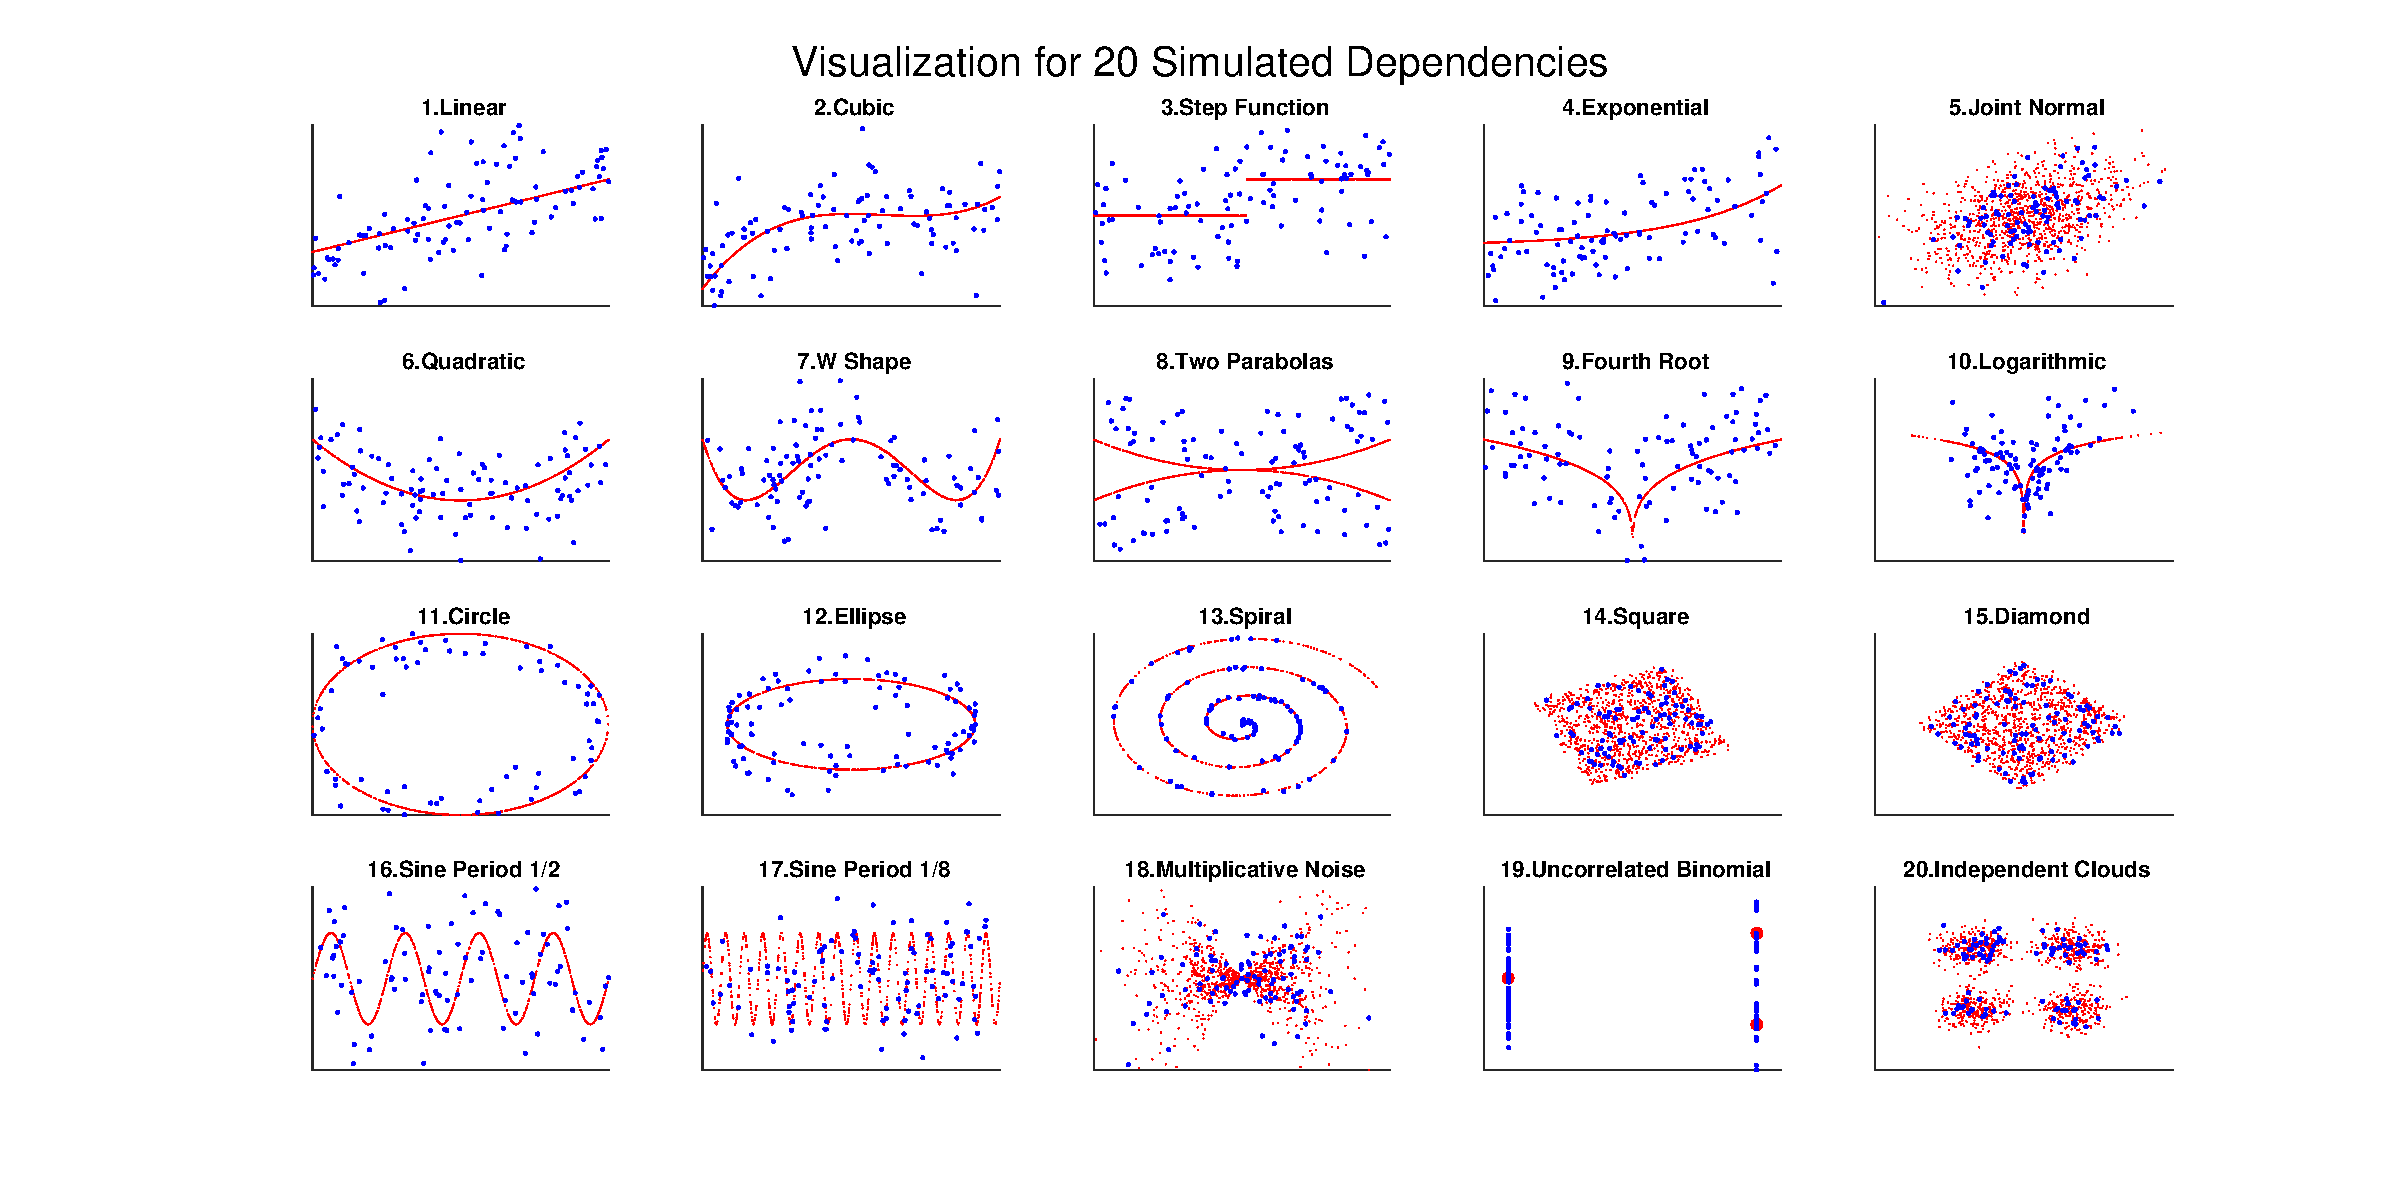
\includegraphics[width=1.0\textwidth]{Figures/Fig0}
	\caption{Visualization of the $20$ dependencies for $1$-dimensional simulations. The blue points are generated with noise (c=1) for $n=100$ to show the actual sample data in testing, and the red points are generated with no noise for $n=1000$ to highlight each underlying dependency.}
	\label{fig1}
\end{figure} 
\end{frame}

\begin{frame}{Simulation Set-Up}
\begin{itemize}[<+->]
\item To calculate the testing power, we repeatedly generate dependent data and independent data from the given model, estimate the test statistic under the null and the alternative, and compute the critical value and power accordingly.
\item We use $10$,$000$ Monte-Carlo replicates to generate the data for testing power computation; and $2$,$000$ additional replicates to generate data for optimal scale estimation.
\item For 1-dimensional simulations, each panel shows empirical testing power on the absicca, and sample size on the ordinate, with dimension fixed at $1$; for high-dimensional simulations, the dimension choice is on the ordinate, with the sample size fixed at $100$.
\end{itemize}
\end{frame}

\begin{frame}{Simulation Interprations}
\begin{itemize}[<+->]
\item We will see that among the benchmarks, dcorr / mcorr can do fairly well in linear problems with mcorr being better in hd linear problems, while HHG works the best in nonlinear problems.
\item Yet MGC achieves the same power as the global correlation under close to linear dependencies, and is equivalent or better than HHG under nonlinear dependencies. This makes MGC the best method throughout all sample sizes / dimensions / simulations (note: different MGC implementations vary slightly in performance, depending on the property of the global correlation).
\item We also show the MGC power heatmap with respect to neighborhood choices, where we can observe that: linear dependency always favors the largest scale (i.e., $\G^{*}=\G$), while nonlinear dependency always favors a smaller scale such that ($\G^{*}>\G$); and similar dependency structure usualy yield similar optimal scales.
\end{itemize}
\end{frame}

\begin{frame}{$1$-Dimensional Testing Powers}
\begin{figure}[htbp]
  \centering
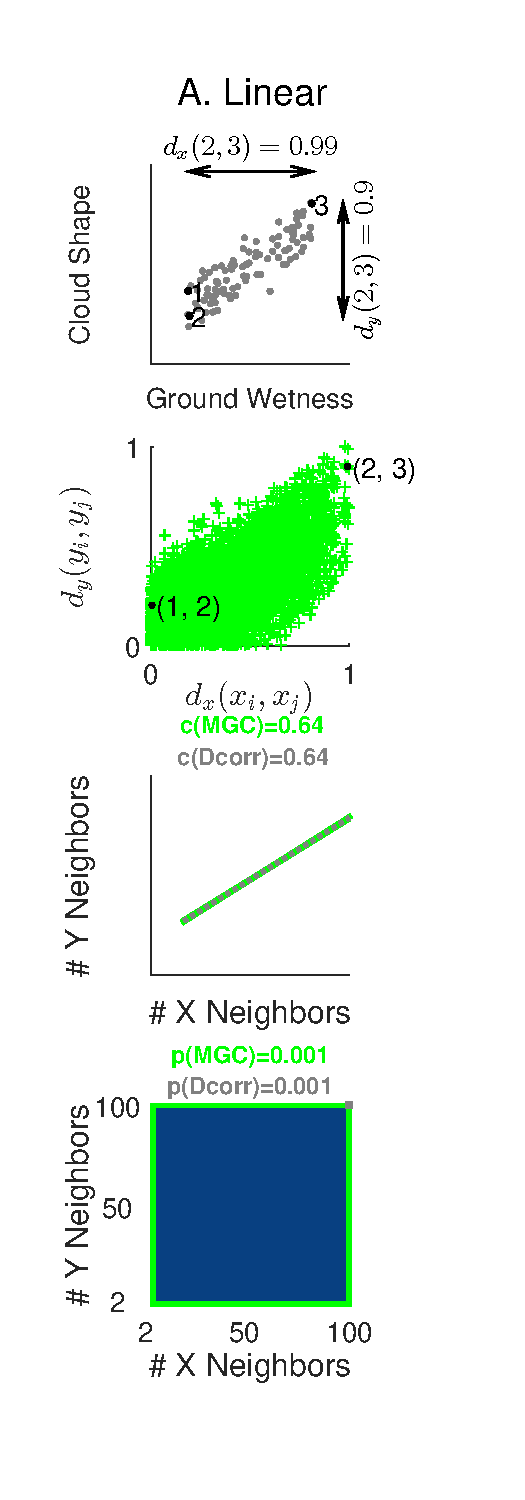
\includegraphics[width=1.08\textwidth]{Figures/Fig1}
\end{figure}
\end{frame}

\begin{frame}{High-Dimensional Testing Powers}
\begin{figure}[htbp]
  \centering
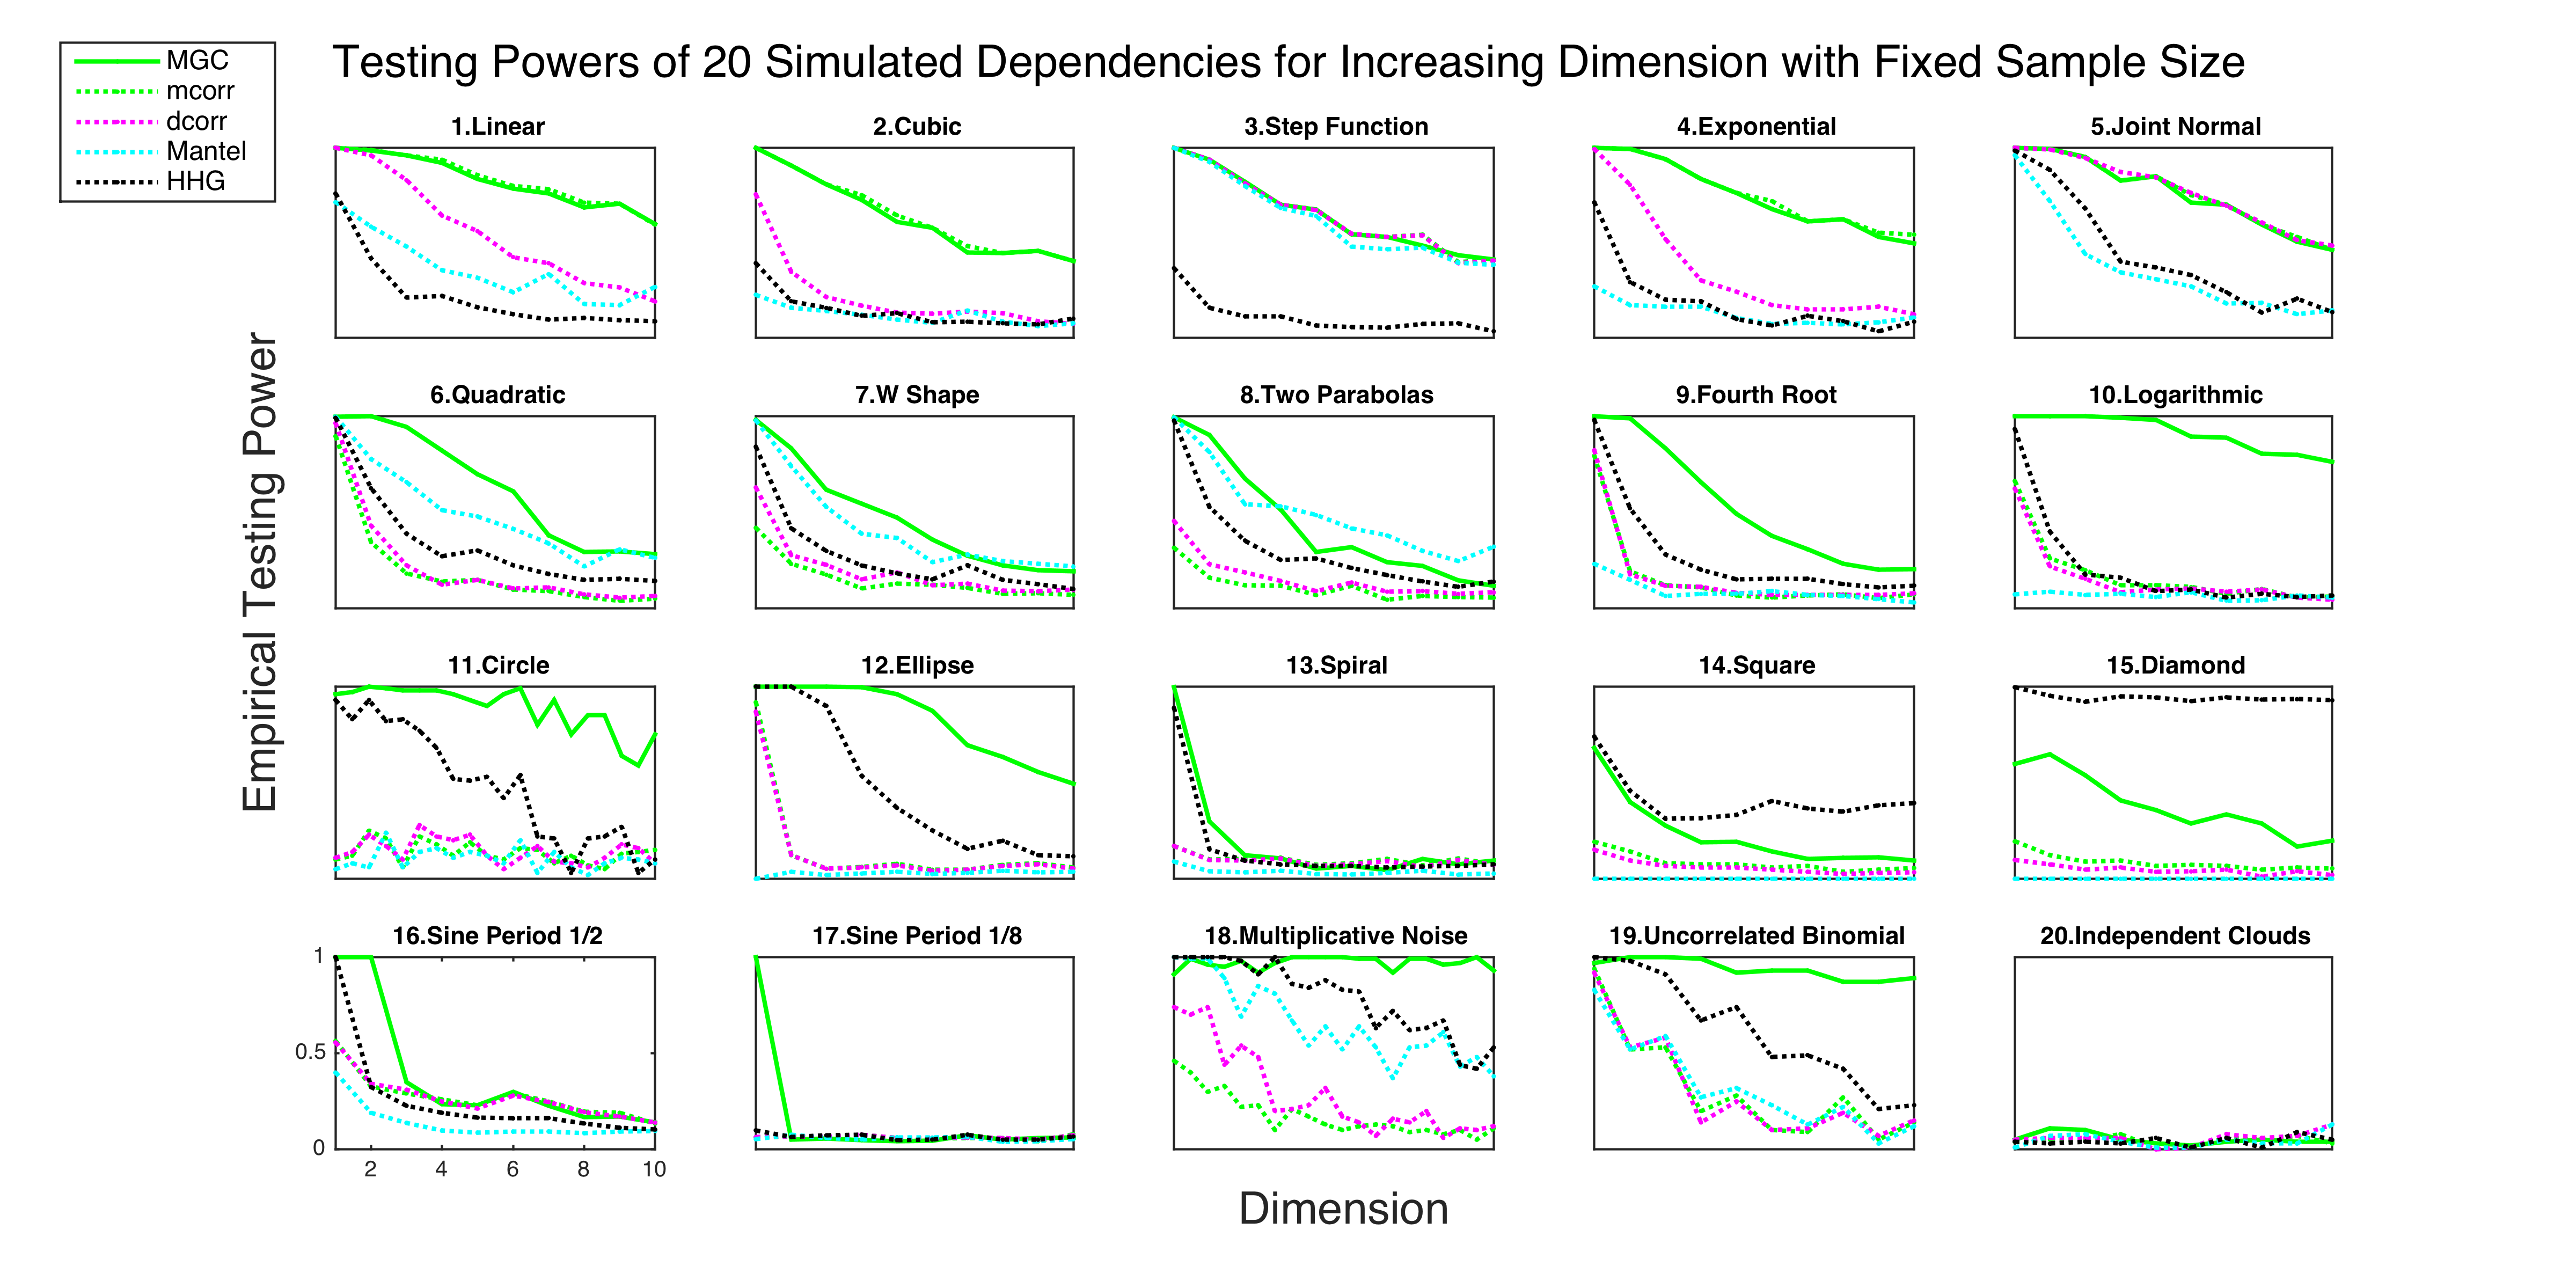
\includegraphics[width=1.08\textwidth]{Figures/Fig5}
\end{figure}
\end{frame}

\begin{frame}{High-Dimensional Local Mcorr Power Heatmap}
\begin{figure}[ht]
  \centering
  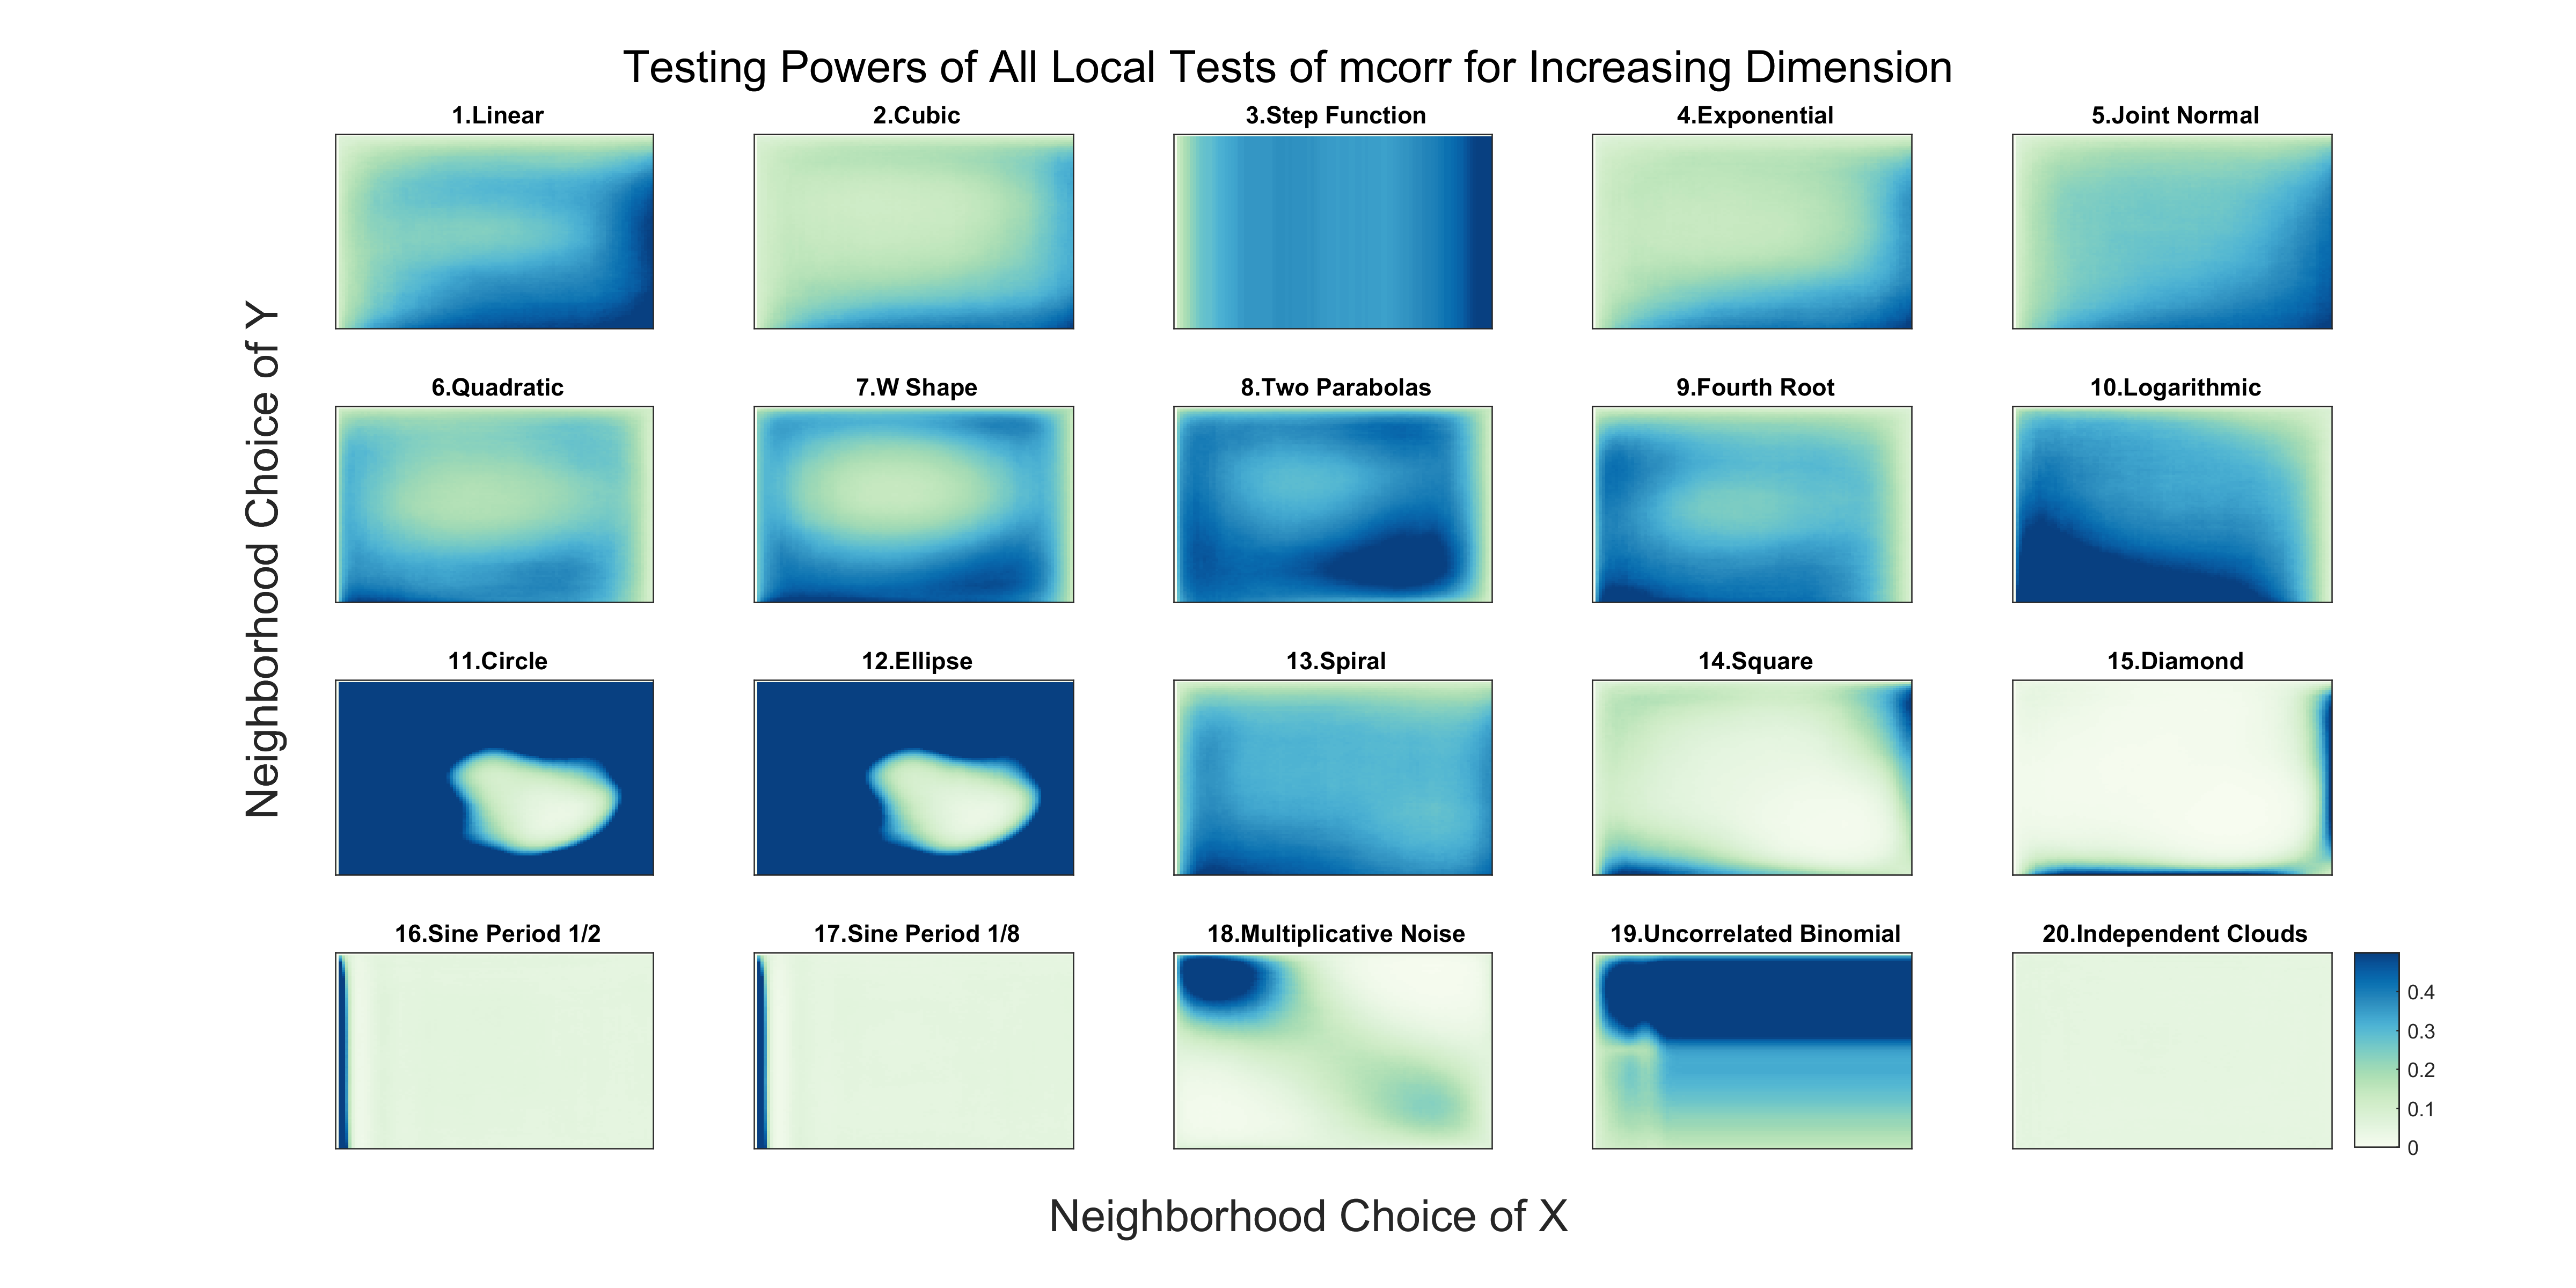
\includegraphics[width=1.08\textwidth]{Figures/Fig6}
\end{figure} 
\end{frame}

\section{Conclusion}
\begin{frame}{Advantages of MGC}
\begin{itemize}[<+->]
\item 1) Easy to implement for any global correlation / any data with a suitable distance metric, and comparable in running time to existing methods.
\item 2) When MGC is based on dcorr/mcorr, MGC is consistent for testing independence.
\item 3) MGC is equivalent to the respective global correlation under linear dependence, but can perform better under nonlinear dependence.
\item 4) Superior numerical performance in a comprehensive simulation setting, including various linear/nonlinear/high-dimensional/noisy dependency.
\item 5) Provides information on the local scale where the dependency is the strongest, and implies the linearity/nonlinearity of the underlying dependency.
\item 6) Does not inflate the false positive rate.
\item 7) MGC is a better scalable method, for big data where distance-based testing method is often performed on sub-samples.
\end{itemize}
\end{frame}

\begin{frame}{What We Do Not Show In Slides}
\begin{itemize}[<+->]
\item MGC is robust against outliers;
\item In case of one pair of given data of unknown model, how to choose the optimal scale heuristically;
\item Real data experiments where MGC is used to detect local signals between brain data vs phenotypes.
\end{itemize}
\end{frame}

\begin{frame}{In The Future}
\begin{itemize}[<+->]
\item Testing dependence on networks.
\item Better optimal scale estimation for unknown model.
\item Investigate alternative form of local correlations.
\item Local correlation is potentially useful for nonlinear embedding, variable selection, etc.
\end{itemize}
\end{frame}

%tba: add PIE and WIKI GF data
%\begin{frame}[allowframebreaks]
%\frametitle{References}
%\tiny
%\bibliographystyle{ieeetr}
%\bibliography{references}

%\end{frame}
\begin{frame}[allowframebreaks]

%\frametitle{References}
\tiny
%\bibliographystyle{ieeetr}
\bibliography{references}

\end{frame}

%------------------------------------------------

%----------------------------------------------------------------------------------------

\end{document} 
